\documentclass[a4paper,12pt]{report}
\usepackage[utf8]{inputenc} % style d'écriture
\usepackage[T1]{fontenc}      % package
\usepackage[francais]{babel}  % package pour langue française
\usepackage[a4paper]{geometry} % definition des marges
\usepackage[pdftex]{graphicx} % definition d'image
\usepackage{fancyhdr} % haut de page
\usepackage{float}
\usepackage{tcolorbox,listings}
\usepackage{caption}
\addtocounter{tocdepth}{3}
\setcounter{secnumdepth}{3}
\usepackage{color}


\lstset{
  aboveskip=5mm,
  belowskip=-2mm,
  basicstyle=\footnotesize,
  breakatwhitespace=false,
  breaklines=true,
  captionpos=b,
  commentstyle=\color{red},
  deletekeywords={...},
  escapeinside={\%*}{*)},
  extendedchars=true,
  framexleftmargin=16pt,
  framextopmargin=3pt,
  framexbottommargin=6pt,
  frame=tb,
  keepspaces=true,
  keywordstyle=\color{blue},
  language=VHDL,
  literate=
  {²}{{\textsuperscript{2}}}1
  {⁴}{{\textsuperscript{4}}}1
  {⁶}{{\textsuperscript{6}}}1
  {⁸}{{\textsuperscript{8}}}1
  {€}{{\euro{}}}1
  {é}{{\'e}}1
  {è}{{\`{e}}}1
  {ê}{{\^{e}}}1
  {ë}{{\"{e}}}1
  {É}{{\'{E}}}1
  {Ê}{{\^{E}}}1
  {û}{{\^{u}}}1
  {ù}{{\`{u}}}1
  {â}{{\^{a}}}1
  {à}{{\`{a}}}1
  {á}{{\'{a}}}1
  {ã}{{\~{a}}}1
  {Á}{{\'{A}}}1
  {Â}{{\^{A}}}1
  {Ã}{{\~{A}}}1
  {ç}{{\c{c}}}1
  {Ç}{{\c{C}}}1
  {õ}{{\~{o}}}1
  {ó}{{\'{o}}}1
  {ô}{{\^{o}}}1
  {Õ}{{\~{O}}}1
  {Ó}{{\'{O}}}1
  {Ô}{{\^{O}}}1
  {î}{{\^{i}}}1
  {Î}{{\^{I}}}1
  {í}{{\'{i}}}1
  {Í}{{\~{Í}}}1,
  morekeywords={*,...},
  numbers=left,
  numbersep=10pt,
  numberstyle=\tiny\color{black},
  rulecolor=\color{black},
  showspaces=false,
  showstringspaces=false,
  showtabs=false,
  stepnumber=1,
  stringstyle=\color{gray},
  tabsize=4,
  title=\lstname,
}

%\captionsetup[figure]{labelformat=empty}
\renewcommand{\thesection}{\Roman{section}}

\begin{document}
   \begin{titlepage}
    
    \newcommand{\HRule}{\rule{\linewidth}{0.5mm}} % Defines a new command for the horizontal lines, change thickness here
    
    \center % Center everything on the page
     
    %----------------------------------------------------------------------------------------
    %	HEADING SECTIONS
    %----------------------------------------------------------------------------------------
    
    \textsc{\LARGE Université de Bretagne Occidentale}\\[1.5cm] % Name of your university/college
		\textsc{\Large Master 2 Informatique}\\[0.5cm] % Major heading such as course name
		\textsc{\Large Département Informatique}\\[1.5cm] % Major heading such as course name
		{\large 2020/2021}\\[1.5cm] % Date, change the \today to a set date if you want to be precise
		
    \textsc{\large Système On-Chip}\\[1cm] % Minor heading such as course title
    
    %----------------------------------------------------------------------------------------
    %	TITLE SECTION
    %----------------------------------------------------------------------------------------
    
   \HRule \\[0.4cm]
    { \huge \bfseries Détection de dépassement de temps d'exécution}\\[0.2cm] % Title of your document
    \HRule \\[1cm]
     
    %----------------------------------------------------------------------------------------
    %	AUTHOR SECTION
    %----------------------------------------------------------------------------------------
    
    \begin{minipage}{0.48\textwidth}
			\begin{flushleft} \large
				\emph{Auteur:}\\
					William \textsc{PENSEC} % Your name
			\end{flushleft}
    \end{minipage}
		~
		\begin{minipage}{0.48\textwidth}
			\begin{flushright} \large
				\emph{Auteur:}\\
					Timothé \textsc{LANNUZEL} % Your name
			\end{flushright}
    \end{minipage}\\[1.5cm]
    
    %----------------------------------------------------------------------------------------
    %	DATE SECTION
    %----------------------------------------------------------------------------------------
    
    {\today}\\[1.5cm] % Date, change the \today to a set date if you want to be precise
    
    %----------------------------------------------------------------------------------------
    %	LOGO SECTION
    %----------------------------------------------------------------------------------------
    
		\begin{minipage}{0.48\textwidth}
			\begin{flushleft} \large
				
\includegraphics[scale=0.8]{ubo_sc.png} % Include a department/university logo - this will require the graphicx package
			\end{flushleft}
    \end{minipage}
		~
    \begin{minipage}{0.48\textwidth}
			\begin{flushright} \large
				
\includegraphics[scale=0.5]{ubo.png} % Include a department/university logo - this will require the graphicx package
			\end{flushright}
    \end{minipage}
    
    %----------------------------------------------------------------------------------------
    
    \vfill % Fill the rest of the page with whitespace
    
    \end{titlepage}
		
	\pagestyle{fancy}
		\lhead{}
		\chead{William PENSEC \& Timothé LANNUZEL}
		\rhead{}
		\lfoot{}
		\cfoot{\thepage}
		\rfoot{}
		
	\newpage\renewcommand{\contentsname}{Sommaire}
	\tableofcontents

	\newpage
	\section{Introduction}
		\paragraph*{}
		L'objectif de ce projet est de concevoir en VHDL un moniteur de temps d'exécution de tâches sur un processeur. En effet, sur un système temps réel, il est très important que les contraintes de temps soient respectées afin d'éviter tout problèmes. Le composant doit suivre l'exécution de chaques tâches et envoyer un signal d'interruption au processeur si l'une d'entre elles dépasse son échéance. La capacité maximale d'une tâche s'appelle le Worst Case Execution Time (WCET). En connaissant cette valeur, on sait si le processeur peut gérer le système ou s'il est nécessaire de le changer pour quelque chose de plus performant.
		
		Afin de simplifier les simulations, nous avons fixé des deadlines de telle manière à ce que tout soit fini en 30 ns maximum lors de la simulation sur Vivado.
		
	\section{Conception VHDL}
		\paragraph*{}
		Le projet s'est découpé en plusieurs étapes qui ont été de créer d'abord les différents modules qui composent le système puis de créer les fichiers de tests (testbench) de ces modules.
		La seconde étape est de regrouper ces modules afin de créer une IP sous Vivado qui pourra être utilisée ailleurs.
		Cette IP sera composée, comme on peut le voir sur l'image \ref{archi}, du CPU, d'une mémoire, de compteurs (module chronomètre) et d'un composant permettant la communication avec le CPU par l'AXI.
		
		\begin{figure}[H]
			\centering
				\includegraphics[scale=0.5]{schemagen.png}
				\caption{Architecture générale}
			\label{archi}
		\end{figure}
		
		\subsection{Chronomètre}
			\paragraph*{}
			L'image \ref{chrono}, à la page \pageref{chrono}, représente le fonctionnement de manière schématique du module chronomètre-décompteur. Le code de cette partie est disponible dans l'archive ou sinon voir le code \ref{chronoCode} à la page \pageref{chronoCode}.
			Le chronomètre est lié à une horloge sur front montant \texttt{rising\_edge(clk)}. Cela permet de contrôler les opérations un front sur deux pour aller un peu plus lentement.
			Autrement, il y a un port de démarrage/arrêt du chronomètre \texttt{startStop} qui permet comme son nom l'indique de démarrer ou stopper le module; mais également un port afin de mettre en pause et de reprendre le timer \texttt{suspendResume}. Nous avons inclu un port de chargement \texttt{load} et de reset \texttt{reset} permettant de charger la valeur d'initialisation (valeur qui correspond à la durée du timer par exemple <10> périodes d'horloge) ou au contraire de mettre à 0 le timer de la tâche en cours.
			
			Enfin, le dernier port qui est celui qui nous intéresse le plus est celui du \texttt{wcet}. Ce port est donc un tableau de 16 bits. C'est dans ce tableau que l'on va enregistrer la valeur du \texttt{Worst Case Execution Time} (\texttt{WCET}). C'est cette valeur qui sera chargée par le port load en mémoire et c'est cette valeur qui servira à décompter le temps avant d'envoyer si besoin l'interruption au processeur si le \texttt{WCET} arrive à 0 dans le timer.
			
			\begin{figure}[H]
				\centering
					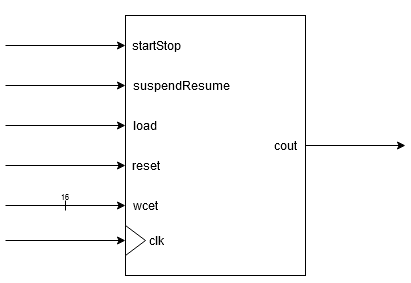
\includegraphics[scale=1]{chrono.png}
					\caption{Bloc chronomètre}
				\label{chrono}
			\end{figure}
			
			
		\subsection{TestBench Chronomètre}
			\paragraph*{}
			Le code du test bench est le code \ref{tbChronoCode} à la page \pageref{tbChronoCode}. Il s'articule de la manière suivante : tout d'abord comme d'habitude nous appellons le component à qui il fait référence, c'est à dire le chronomètre. Puis, on crée les signaux nécessaires pour assigner des valeurs aux ports du composant. Ensuite dans l'architecture comportementale du composant test, on affecte des valeurs aux signaux. Nous avons décidé de faire une horloge avec une période de 1 ns afin d'avoir quelque chose de rapide. La valeur \texttt{startStop\_ch} est initialisée à 0 et passe à 1 après 5 ns c'est à dire que le chronomètre ne démarrera qu'après 5 ns d'exécution de programme, cette valeur a été mise seulement dans un but de test mais en soit doit être initialisée à 1 lors de la création du chronomètre. La valeur \texttt{load\_ch} correspondant au chargement du \texttt{WCET} en mémoire; il est initialisé à 1, c'est à dire qu'on charge en mémoire la donnée dès qu'elle est disponible puis on passe cette valeur à 0 car on désire arrêter la mise en mémoire de la valeur afin de passer à la décrémentation. La valeur du \texttt{reset} est laissé à 0 car nous n'en avons pas besoin du tout mais si on passe cette valeur à 1 alors la donnée est mise à 0 comme convenu ! Enfin, la valeur du \texttt{wcet\_ch} est initialisée à 7.
			
			Un exemple d'exécution est proposé à l'image \ref{chronoTB} à la page \pageref{chronoTB}. On distingue sur l'image toutes les étapes citées dans le paragraphe précédent.
			
		\subsection{Moniteur de tâches}
			\paragraph*{}
			Le moniteur de tâches, comme on peut voir sur l'image \ref{moniteur} à la page \pageref{moniteur}, possède 1 port de sortie et 5 ports d'entrées. Comme sur le chronomètre, il y a l'horloge et le reset. Le port \texttt{id\_task} correspond à l'ID sur 4 bits de la tâche en cours, par exemple, si \verb|id_task = 0001| alors ça veut dire que la tâche en train de s'exécuter est la tâche 1. Le port \texttt{mess\_task} correspond au message d'exécution, il peut prendre des valeurs entre 0 et 5. Le détail des valeurs possible est :
			
			
			\begin{description}
				\item[0 : ] 'stop'
				\item[1 : ] 'start'
				\item[2 : ] 'load'
				\item[3 : ] 'suspend'
				\item[4 : ] 'resume'
				\item[5 : ] 'reset'
			\end{description}
			
			Le port \texttt{wcet\_task} correspond à la donnée de temps maximal d'exécution qui doit ensuite être décrémenté lors de l'exécution de la tâche par le module chronomètre.
			Enfin, le port de sortie \texttt{counter\_interupt} est à 0 tout le temps et doit rester à 0 car s'il passe à 1 cela veut dire qu'une tâche à dépasser son temps d'exécution et donc un signal d'interruption doit être envoyé au processeur !
			
			\begin{figure}[H]
				\centering
					\includegraphics[scale=0.5]{moniteur.png}
					\caption{Bloc représentant le moniteur de tâches}
				\label{moniteur}
			\end{figure}
	
		\subsection{TestBench Moniteur de tâches}
			\paragraph*{}
			Le testbench du moniteur de tâches sert juste à simuler le programme en créant 2 tâches (la tâche 0 et la tâche 1) et en les exécutant en regardant si le chronomètre arrive à 0 ou non. L'image \ref{monitorTB} à la page \pageref{monitorTB} permet de voir que les 2 tâches que l'on a exécuté s'exécutent bien et que la tâche 0 ne se termine pas alors que la tâche 1 est fini en une période d'horloge.
			
			La tâche 0 ne respecte pas son WCET car la valeur de \texttt{compteur\_test} arrive à 0 au bout de 18 ns, le signal d'interruption est bien envoyé aussi car la variable \texttt{compteur} passe bien à 1 lorsque le chronomètre arrive à 0.
			
			Les tâches sont contrôlées avec la variable \texttt{message} qui change de valeur de temps en temps pour tester un cas possible d'exécution.
						
						
	\section{Résultats}
		\subsection{Chronomètre}
			\paragraph*{}
			Comme on peut voir sur cette image, le signal \texttt{clk\_ch} correspondant à l'horloge du CPU oscille chaque nanoseconde.
			
			Dans l'ordre du temps, tout d'abord à 0 ns on a en mémoire le wcet de la tâche, cette valeur est initialisée dans la variable de sortie test 'cout\_test\_ch' à 1 ns qui correspond au front montant de l'horloge. Après 4 ns, le \texttt{load\_ch} passe à 0 ce qui permet d'arrêter la mise en mémoire du wcet en continu, si cette variable était resté à 1 le chronomètre ne se serait jamais lancé. La variable \texttt{startStop} lance l'exécution du module à 5 ns et le décompte commence aussitôt sur la sortie. Enfin, au bout de 17 ns, on voit que la variable \texttt{cout\_ch} passe à 1 ce qui signifique que le chronomètre est arrivé à 0 et qu'il est nécessaire au module supérieur de lancer le signal d'interruption au processeur.
			
			Nous avons ajouté un port de sortie \texttt{cout\_test\_ch} qui permet de lire les résultats plus simplement.
			
			\begin{figure}[H]
				\centering
					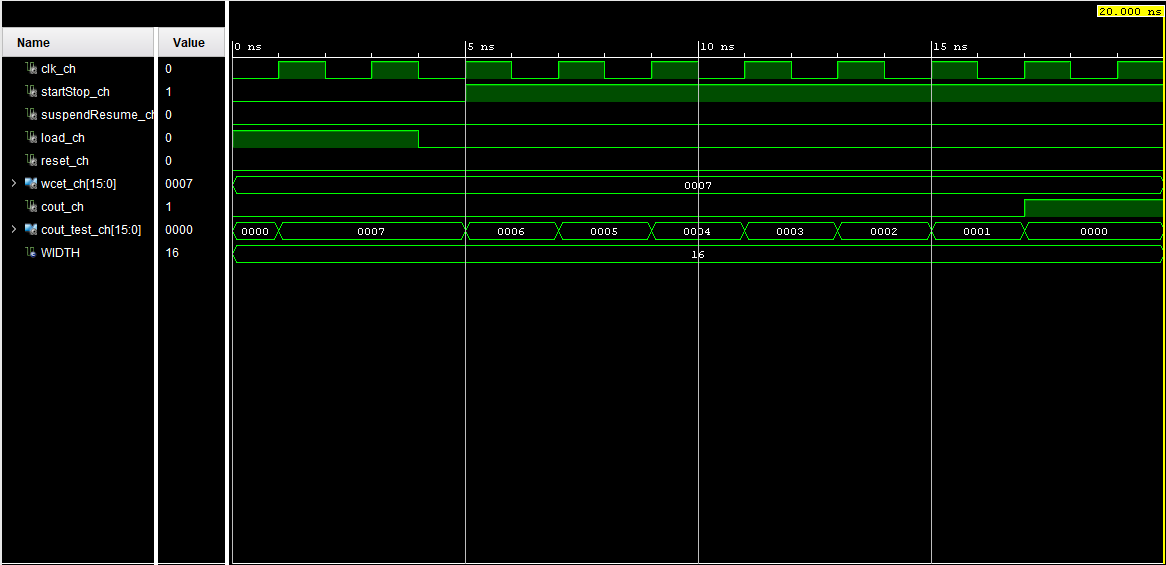
\includegraphics[scale=0.5]{chrono_tb.png}
					\caption{Testbench chronomètre}
				\label{chronoTB}
			\end{figure}
			
		\subsection{Moniteur de tâches}
			\paragraph*{}
			L'image suivante correspond à l'exécution du composant \texttt{taskMonitor} avec 2 tâches en entrée possédant respectivement un WCET de 3 et de 5.
			
			L'ordre d'exécution par rapport au temps est tout d'abord le message est à 0 donc l'état de la tâche 0 comme indiqué avec l'ID à 0 est sur stop, à 1 ns (période de l'horloge), le WCET de la tâche 0 est initialisé à 0 car l'instruction de chargement 'load' n'a pas été reçu. Cette instruction arrivera au bout de 2 ns. Le troisième message reçu est le 'start' à 3 ns mais le programme ne commencera qu'au tick suivant c'est à dire 4 ns. Le décompte commence donc de 3 puis passe à 2 avant d'être stoppé à 7 ns pour laisser la main à la tâche 1 qui s'exécute de 10 ns à 12 ns et puis la tâche 0 reprend jusqu'à arriver à 0 au bout de 17 ns et donc d'envoyer le signal d'interruption immédiatement au processeur. Nous pouvons voir que la tâche 0 reprend bien à 2 et non pas au départ donc on a bien une sauvegarde de la valeur et un chargement correct sans le reset.
			
			Nous avons ajouté un port de sortie \texttt{compteur\_test} qui prend la valeur de \texttt{cout\_test\_ch} qui permet de lire les résultats de la tâche courante plus simplement.

			\begin{figure}[H]
				\centering
					\includegraphics[scale=0.4]{moniteur_tb.png}
					\caption{Testbench moniteur de tâches}
				\label{monitorTB}
			\end{figure}
	
	\section{Continuité du projet}
		\paragraph*{}
		La première étape serait de réaliser l'IP sur Vivado avec les branchements AXI et ensuite de générer le block design complet 
		
		La deuxième étape serait de générer le fichier 'wrapper' dont le rôle est de connecter les Entrées/Sorties sur les broches physiques du FPGA.
		
		La troisième étape serait de lancer la synthèse et implémentation du programme Vivado, créer le bitstream.
		
		Enfin, la dernière étape serait la réalisation d'un programme en C dans le but d'interfacer ce même programme et le code VHDL afin de générer les tâches et envoyer ces id, messages et autres données au code moniteur de tâches puis au chronomètre. Et enfin, exécuter le code sur un FPGA afin de tester son bon fonctionnement.
	
	
	\section{Code}
		\subsection{Chronomètre}
			\lstinputlisting[caption={Chronomètre}, label={chronoCode}]{"../Projet_SOC/Projet_SOC.srcs/sources_1/new/chronometer.vhd"}
		
		\subsection{TestBench Chronomètre}
			\lstinputlisting[caption={TestBench chronomètre}, label={tbChronoCode}]{"../Projet_SOC/Projet_SOC.srcs/sim_1/new/chronometer_tb.vhd"}
			
		\subsection{Moniteur de tâches}
			\lstinputlisting[caption={Moniteur de tâches}, label={taskMonitorCode}]{"../Projet_SOC/Projet_SOC.srcs/sources_1/new/taskMonitor.vhd"}
		
		\subsection{TestBench Moniteur de tâches}
			\lstinputlisting[caption={TestBench moniteur de tâches}, label={tbMonitorCode}]{"../Projet_SOC/Projet_SOC.srcs/sim_1/new/tasksMonitor_tb.vhd"}
			
			
	\clearpage
\end{document}